\chapter[The Standard Model]{The Standard Model}
\label{chap:SM}
Since the Greeks, different theories about the composition and structure of the world have been formulated. At ancient Greece these theories were elaborated from a philosophical point of view. Nowadays, we count with a very sophisticated  set of tools and concepts that allowed us to build up a general vision of nature, its components and structure. Moreover, on the subject of the constituents, or elemental constituents, a theory capable of describing the majority of known phenomena has been developed. This theory is the Standard Model (SM) of particle physics. 

This SM relies in two of the more elegant constructs of modern physics and mathematics. From the physics side, the quantum field theory; from mathematics, group theory. Quantum field theory has born from the understanding of processes that take place at very small spatial scales and in a regime where special relativity play an important role. To describe such, a major part of the most brilliant minds of the 20th century dedicated their life, Paul Dirac, Richard Feynman, Enrico Fermi among them. The theory of quantum fields has set in a common place two extraordinary achievements of physics: special relativity and quantum mechanics. With it we have been capable to describe many phenomena: $\beta$ and $\alpha$ decay, solid state, among many other.

From the mathematics side, group theory has become one of the most powerful tools for particle physicist. However, their development began quite early, with Galois around 1830, and was used in other parts of physics, it's with Lie algebras and the possibility of describing continuous symmetries that the most important step were given. Also, this would have not been possible with the amazing connection found by Emmy Noether in 1918. She found that for every conserved quantity there is a preserved symmetry. Group theory can be seen, roughly speaking, a way to mathematically describe symmetries, group theory became the tool to describe systems with conserved quantities. 

In this chapter, we present the basics of the SM. We describe its seminal ideas, it structure and content and it's ultimate consequences. Finally, we close with its limitations.

\section{Fields, symmetries and interactions}
\label{sec:symm}

From the very beginning of physics, one of the most fundamental questions has been how does bodies interact, and what is exactly an interaction. On the first type of interaction ever studied by physics, gravity, Newton proposed the concept of distant interaction, the idea that bodies could interact without being in direct contact. But the question on how exactly that distant action was performed remained unanswered. 

During the 19th and 20th century new phenomena were discovered pointing to brand new interactions, electricity, magnetism and radioactivity. The very precise and complete description of electromagnetism developed by Gauss, Faraday, Amp\`{e}re and finished by Maxwell arrived to describe electricity and magnetism under the formalism of only one interaction within the mathematical formalism of classical fields. Further works addressed radioactivity, driving to a deeper understanding of nature and it composition.

For the following discussion, and later, we are going to work in natural units for simplicity. In these units the speed of light $c$ is normalized to unity, as well as electron electric charge $e$, reduced Planck constant $\hslash$ and Boltzmann constant $k_{B}$. Then, masses and temperature are expressed in energy units, i.e. $eV$, and time and length in inverse energy units, $eV^{-1}$.

A classical field is an assignment of a quantity to every point in space and time. For physics, the quantity that is attributed it is a physical quantity such as mass, electrical charge or probability. This quantity can be scalar or vector, giving rise to the notion of scalar or vector field, correspondingly. The simplest example, is the temperature in a gas, that is a scalar quantity assigned to every point. Another example, a fluid can be described in terms of fields, being the velocity of the fluid a vector field and its pressure a scalar field. Generic classical electromagnetic interactions can be described with the help of one vector field $\vec{A}(x)$, the vector potential, and one scalar field $\phi(x)$, the scalar potential. In the formalism of four-vectors from relativistic dynamics one can organize this two quantities in the four-potential $A_{\mu}=(-\phi,\vec{A})$. This can be used to define the strength field tensor $F_{\mu\nu}=\partial_{\mu}A_{\nu}-\partial_{\nu}A_{\mu}$, where $\partial_{\mu}=\left( -\frac{\partial}{\partial t},\nabla\right)$ is the covariant derivative. From the tensor is possible to obtain in a very generic and elegant way the equations of motion of the free field using the Lagrangian formalism, as in equation~\ref{eq:electromotion}. With the Lagrangian density defined in equation~\ref{eq:electrolagran}.

\begin{equation}
  \label{eq:electromotion}
  \partial_{\mu}\left( \frac{\partial \mathcal{L}}{\partial (\partial_{\mu}A_{\nu})} \right) -\frac{\partial \mathcal{L}}{\partial A_{\nu}}=0
\end{equation}

\begin{equation}
  \label{eq:electrolagran}
  \mathcal{L}=-\frac{1}{4}F^{\mu\nu}F_{\mu\nu}
\end{equation}

It's very important to notice that the equations of motion of the free field are invariant under the choice of the four-potential. More precisely, the covariant potential is not unique and we can always add the covariant derivative of a scalar field, 
\begin{equation}
  \label{eq:gaugeA}
  {A'}_{\mu}=A_{\mu}+\partial_{\mu}\Lambda(x) \leftrightarrow \partial^{\mu}A_{\mu}=0
\end{equation} and describe the same physics. This non-uniqueness corresponds to the choice of a zero-point of the potential very well known in non-Lagrangian formalism of electrodynamics. When we choose a specific value for this scalar field, $\Lambda(x)$, we say that the gauge has been fixed. 

One can also define a four current vector, $J_{\mu}=\left( \rho,\vec{J} \right)$ with $\rho$ the electric charge density and $\vec{J}$ the current charge density. Then, plugging in this four current in the Lagrangian of the free field, defined in equation~\ref{eq:electrolagran}, 

\begin{equation}
  \label{eq:fulleleclagrangian}
  \mathcal{L}=-\frac{1}{4}F^{\mu\nu}F_{\mu\nu}-A_{\mu}J^{\mu}
\end{equation}we can obtain the complete set of equations of motion of the field with charges and currents. 

The transformation stated from equation~\ref{eq:gaugeA} can be understood as a transformation of the field. These type of transformations are mathematically understood under the group $U(1)$, where the generic transformation operator can be written as $U=e^{i\theta(x)}$. It's said then that the electromagnetic vector potential is \textit{invariant} under $U(1)$ transformations. This property identifies an essential characteristic of electromagnetism, its symmetric behavior under $U(1)$. 

From this reasoning the most interesting results are drawn when the same symmetry is imposed to another fields. For example, the kinetic Lagrangian for a complex scalar field is $\mathcal{L}=(\partial^{\mu}\phi)^{*}\partial_{\mu}\phi$. To perform the transformation on the scalar field, it is sufficient to apply the operator as $\phi'=U\phi$ and ${\phi'}^{*}={\phi}^{*} U^{-1}$. But it's evident that the Lagrangian is not the same after applying such transformation. Then, in order to preserve the Lagrangian under $U(1)$ is necessary to change at the same time the derivative. Such transformation is given in equation~\ref{eq:covderivU1}, where $g$ is a constant.

\begin{equation}
  \label{eq:covderivU1}
  \mathcal{D}^{\mu}=\partial^{\mu}-igA^{\mu}
\end{equation}

Then, the proposed Lagrangian can be rewritten, including the vector field, as

\begin{equation}
  \label{eq:FullLagU1inv}
  \mathcal{L}=(\mathcal{D}^{\mu}\phi)^{*}\mathcal{D}_{\mu}\phi-\frac{1}{4}F^{\mu\nu}F_{\mu\nu}
\end{equation}that is invariant under $U(1)$. An interaction term, of the form $igA^{\mu}\phi^{*}\partial_{\mu}$, between the scalar and the vector field, can be derived from the kinematic part of the Lagrangian $\mathcal{D}^{\mu}\phi)^{*}\mathcal{D}_{\mu}\phi$. This shows that the requirement of the invariance under $U(1)$ of the scalar field lead to the introduction of an interaction with a vector field controlled by the constant $g$. We have also seen that electromagnetic interaction is described precisely by a vector field and that preserves $U(1)$ symmetry, which implies that this symmetry is the connection to electromagnetic interaction, identifying the interaction itself with the $U(1)$ symmetry. In addition, using Noether theorem one can show that $g$ is a conserved quantity, as the electric charge is.

But not only electromagnetism can be described via a continuous symmetry as $U(1)$. On 1896 radioactivity was discovered by the french physicist Henri Becquerel. Three years after, Marie and Pierre Curie studied in more detail the phenomenon and found Polonium and Radium elements. And later on, Ernst Rutherford was able to describe radioactivity as coming in three types, alpha ($\alpha$), beta ($\beta$) and gamma ($\gamma$). He also noticed that radioactivity was able to change matter, which allowed him, with also other experiences, to propose an atomic model, describing elements as basically and external core of negative charges and a nucleus positively charged. Consequently, This findings implied the existence of interactions different to electromagnetism, acting at the atomic scale.

The interaction that undergoes radioactivity, beta decay, is called the weak interaction. In 1933 Enrico Fermi made a first theoretical description of this interaction, but only in 1968 Sheldon Glashow, Abdus Salam and Steven Weinberg were able to describe weak interaction with a symmetry group: $SU(2)$. Finally, the interaction that keeps the nucleus components together, the strong interaction, was described with $SU(3)$ group mainly by Murray Gell-Mann in 1963.

There have been many attempts to describe gravity with the same formalism, but up to present such attempts have been unsuccessful. Such question remains one of the most important problems for modern particle physics.  

\section{Quantum fields and particles}
\label{sec:fields}

Classical fields, introduced and described in last section~\ref{sec:symm}, can be extended to a quantum theory. Such procedure is known as the quantization of fields and allow to unify special relativity and quantum mechanics in one theory, Quantum Field Theory (QFT), to describe the dynamics of systems in such regimes: speed close to the speed of light on the atomic or smaller scales.

Quantum mechanics introduced two fundamental concepts: first, the description of the system by its states; and second, the identification of an observable with an operator. The state of a system is identified with a set of quantum numbers that tell us the characteristics of the system when is at some state. For example, the hydrogen atom system has energy as quantum number, such that each state has a value for the energy describing the potential energy contained in the system. Quantum states are mathematically noted in Dirac notation as a \textit{ket},

\begin{equation}
  \label{eq:DiracNot}
  \ket{\alpha}=\ket{i,j,k,\dots}
\end{equation}with $\alpha$ the set of quantum numbers $i,j,k,\dots$ This mathematical object lives in Hilbert space (a complex space $\mathds{C}$ of functions), which conjugate, a \textit{bra}, is noted $\bra{\alpha}$, and their internal product $\braket{\beta}{\alpha}$. The numerical value of $|\braket{\beta}{\alpha}|^{2}$ gives the transition probability of the system from state $\beta$ to state $\alpha$, and $|\braket{\alpha}{\alpha}|^{2}$ is the probability to find the system in state the $\alpha$.

Physical observables as position, energy or momentum are described by complex operators such that to measure their value for a given state, one just have to calculate $|\bra{\alpha}\hat{O}\ket{\alpha}|^{2}$. The identification of observables and operators is called \textit{first quantization}. In addition, Schrodinger equation describes the evolution of states,

\begin{equation}
  \label{eq:Schrodinger}
  \hat{\mathcal{H}}\ket{\alpha}=i\frac{d}{dt}\ket{\alpha}
\end{equation}with $\mathcal{H}$ the Hamiltonian of the system. The whole formalism is able to explain \textit{quantized} systems, where the quantum numbers are discrete, such as hydrogen atom or black body.

Several functions or fields can be related to a given state. These functions, wave functions, can be used as the states to calculate probabilities. In \textit{second quantization} wave functions are upgraded into field operators. This procedure gives rise to the quantization of the state of the field, which is described by the quantum number $n$ which is definite positive. $n=0$ for the fundamental state and $n>0$ for the excited states. Such excitations of the field are understood as physical particles that propagates in space-time, which means that $n=0$ is vacuum. 

The first QFT ever created was born from the quantization of the electromagnetic field. Quantum Electro Dynamics (QED) is the quantized version of classical electrodynamics, that was developed by Tomonaga, Schwinger and Feynman around 1960. This theory describes electromagnetic interactions of a charged field and the electromagnetic vector field. The charged field excitations correspond to electrons and the excitations of the vector fields are photons, responsible of light. Electrons are a particle with negative electric charge and orbit around the nucleus in atoms. Discovered in 1897 by J. J. Thomson, it was fully described by P. A. Dirac in 1928 with the Dirac equation that is the Schrodinger equation for a relativistic particle of spin 1/2. Spin, the intrinsic angular momentum carried by a particle, can be integer (0,1,2,...) or semi-integer ($\frac{1}{2}$,$\frac{3}{2}$,...). The particles with semi-integer spin, as electrons, are called \textit{fermions} and particles with integer spin, as photons, are called \textit{bosons}. Dirac equation predicted the existence of a particle identical to the electron but with positive charge, the positron. It was discovered on 1932 by Carl David Anderson.

Up to present days we have found 12 fundamental fermions and 5 fundamental bosons. Fermions are organized in \textit{leptons}, that don't interact strongly, and \textit{quarks}, that do interact strongly. Leptons are as well organized in three families, the electron ($e^{-}$) and electron neutrino ($\nu_{e}$), muon ($\mu^{-}$) and muon neutrino ($\nu_{\mu}$) and tau ($\tau$) and tau neutrino ($\nu_{\tau}$). Electron, muon and tau are electrically charged while neutrinos are neutral. Their respective anti-particles are equally organized, positron ($e^{+}$) with electron anti-neutrino ($\bar{\nu}_{e}$), anti-muon ($\mu^{+}$) with muon anti-neutrino ($\bar{\nu}_{\mu}$) and anti-tau ($\tau^{+}$) with tau anti-neutrino ($\bar{\nu}_{\tau}$). Quarks also come in three families, with the respective anti-quarks: up ($u$, $\bar{u}$) and down ($d$, $\bar{d}$), charm ($c$, $\bar{c}$) and strange ($s$, $\bar{s}$), top ($t$, $\bar{t}$) and bottom ($b$, $\bar{b}$). The fundamental bosons are the photon (A), the W (positively and negatively charged) and Z that mediate the electroweak interaction, the gluon ($g$) mediating the strong interaction and the Higgs ($H$). The weak bosons were discovered at CERN in 1983 at the UA1 and UA2 collaborations over the SPS accelerator (described on section~\ref{sec:injector}). The Higgs boson has been discovered recently on 2012 by ATLAS and CMS experiments at the LHC. The 2013 physics Nobel prize was awarded to Francois Englert and Peter W. Higgs "for the theoretical discovery of a mechanism that contributes to our understanding of the origin of mass of subatomic particles, and which recently was confirmed through the discovery of the predicted fundamental particle, by the ATLAS and CMS experiments at CERN's Large Hadron Collider".

\subsection{The mass problem}
\label{sec:mass}

Using the concepts developed on later sections about QFT and symmetries it's possible to construct a whole theory giving rise to a precise description of particles and interactions between them. But such a theory does not allow to have massive bosons, whereas masses for fermions are allowed. A mass term for a fermion $\psi$ is of the form 

\begin{equation*}
%  \label{eq:elemass}
  m_{\psi}\bar{\psi}\psi
\end{equation*} where $m_{\psi}$ is the mass of the field.

Under $U(1)$ transformations, $\psi'=U \psi$, the mass term remains the same, what means that is invariant under $U(1)$ transformations. The same is not true for a boson. A mass term for a boson $A$, can be written as 

\begin{equation}
  \label{eq:Amass}
  m_{A}A^{\mu}A_{\mu}
\end{equation} where $m_{A}$ is its mass.

The $U(1)$ transformation for the boson is $A'^{\mu}=A^{\mu}+\delta^{\mu}\theta(x)$. Applying such transformation on the mass term~\ref{eq:Amass} one can obtain the transformed term

\begin{equation}
  \label{eq:Amass}
  m_{A}\left(A^{\mu}A_{\mu}+A^{\mu}\delta_{\mu}\theta(x)+\delta^{\mu}\theta(x)A_{\mu}+\delta^{\mu}\theta(x)\delta_{\mu}\theta(x)\right)
\end{equation}where the last three terms make this term not invariant under $U(1)$ transformations. Consequently, one can say that a mass term for the boson destroy the invariance of the theory under $U(1)$ symmetry.

Nonetheless there is no need for a theory of a massive photon, there is a need to have massive bosons for weak interactions. There is a relation between the mass of a boson and the range of the interaction mediated by it. Massless bosons transmit long range interactions, as electromagnetism, but short range interactions, as the weak interaction, are mediated by massive bosons. More precisely the interaction range is inversely proportional to the mass of the boson, higher the mass shortest the range. Such relation can be seen from the structure of the propagator, which is a mathematical entity that describes the probability a particle has to travel a distance in a given time. Such propagator, for a vector boson, has a generic form given in equation~\ref{eq:Propa}, where $k_{\mu}$ is the momentum carried by the boson. It's clear from this structure that a massive boson has less probability to travel a long distance than a massless boson in a given time.

\begin{equation}
  \label{eq:Propa}
  \frac{g_{\mu\nu}}{k^{2}-m^{2}+i\epsilon}
\end{equation}

Then, as massive bosons are requires for weak interaction, somehow the $SU(2)$ symmetry has to be broken. There are basically two ways to broke a symmetry: 
\begin{itemize}
\item Explicit symmetry breaking: By the introduction of a symmetry breaking term in the Lagrangian, as a mass term for the bosons.
\item Spontaneous symmetry breaking: When the ground state of one field fail to be invariant under the symmetry. 
\end{itemize}

Explicit symmetry breaking is not an option, because the symmetry needs to be preserved in the Lagrangian in order to introduce the interaction.

\subsection{Spontaneous Symmetry Breaking}
\label{sec:SSB}

Several physical systems exhibit an spontaneous symmetry breaking. For example, a pencil balanced on its tip is perfectly symmetric system around the vertical axis, however, because of the instability of the system the pencil will eventually fall over. The final state is stable but not symmetrical. This transition also decreased the potential energy of the system, driving the system to its ground state. This means that whereas the system had a symmetry the ground state does not show the symmetry. In general, symmetry breaking is linked to phase transitions, as liquid to gas transition or magnetization of a ferromagnet, covering a plethora of physical processes. To a greater extent, in recent studies,~\cite{2015arXiv150302776M}, the emergence of life has been understood as a phase transition of matter. 

To achieve an spontaneous symmetry breaking of $SU(2)$ in QFT one should choose a field for which its ground state, vacuum, will fail the symmetry. This means, in practical terms, that such field will have a non-zero value in vacuum, leading to a presence of particles coming from the field on theory vacua. If a fermion field is chosen, the vacuum will show a preference on directionality depending on its spin orientation, what breaks Poincar\'{e} symmetry imposed by special relativity. The same is true if a spin-1 bosonic field is chosen for the task. In order to avoid this problem a spin-0 field should be used. In addition, this field should be electrically neutral to avoid having a charged vacuum.

Whit all this properties in mind, taking a scalar doublet of $SU(2)$, defined on equation~\ref{eq:HiggsDoublet} where $\phi^{0}$ and $\phi^{+}$ are complex fields, the most general potential can be written from two auto-interaction terms, in equation~\ref{eq:HiggsPotential}.

\begin{equation}
  \label{eq:HiggsDoublet}
  \Phi=\left(
    \begin{array}{c}
      \phi^{+} \\
      \phi^{0}
    \end{array}
  \right)=\left(
    \begin{array}{c}
      \phi^{+} \\
      \phi_{RE}-i\phi_{IM}
    \end{array}
  \right)
\end{equation}

\begin{equation}
  \label{eq:HiggsPotential}
  V(\Phi)=\mu^{2}\Phi^{\dagger}\Phi+\lambda(\Phi^{\dagger}\Phi)^{2}
\end{equation}

Such potential has a unique minimum for $\lambda>0$ and $\mu^{2}>0$, but for $\lambda>0$ and $\mu^{2}<0$ has a set of minima with the shape of ``Mexican hat'', shown in figure~\ref{fig:MexicanHat}. Under $\lambda>0,\;\mu^{2}<0$ configuration the field breaks spontaneously the symmetry reaching the ground state, acquiring an expectation value on vacuum different from zero, $v$. 

\begin{figure}[!Hhtbp]
  \begin{center}
    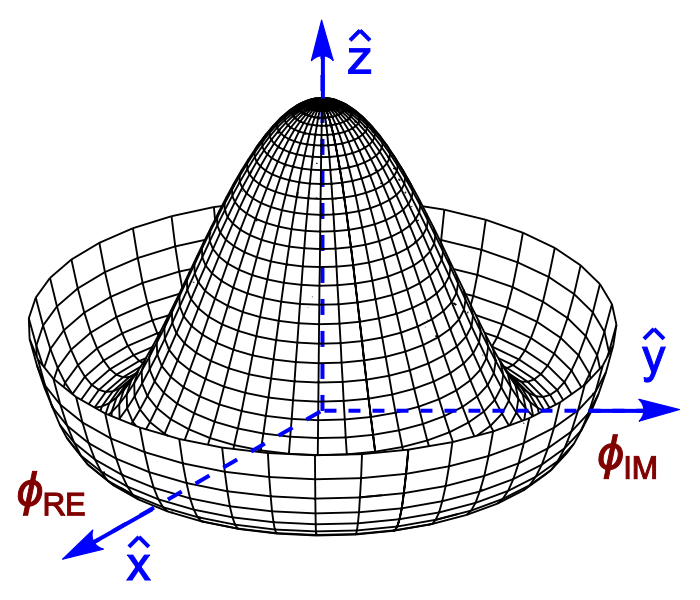
\includegraphics[width=0.6\textwidth]{figs/Mexican_hat.png}
    \caption{Higgs potential}
    \label{fig:MexicanHat}
  \end{center}
\end{figure}

\subsection{Englert-Brout-Higgs mechanism}
\label{sec:higgs}

After the spontaneous symmetry breaking, the scalar doublet transforms into the form given in equation~\ref{eq:TransHiggsDoublet}, where $G^{+}$ and $G^{0}$ are the Goldstone bosons product of the breaking of the $SU(2)$ symmetry, and $H$ is the Englert-Brout-Higgs boson. From Goldstone's, theorem when a symmetry is spontaneously broken a massless boson appear for each broken generator. In our specific case, the three generators of $SU(2)$ are broken giving rise to three Goldstone bosons: $G^{+}$, $G^{-}$ and $G^{0}$. This massless bosons are ``eaten'' by the $W^{+}$, $W^{-}$ and $Z^{0}$ giving them an additional degree of freedom, the longitudinal polarization. 

\begin{equation}
  \label{eq:TransHiggsDoublet}
  \Phi=\left(
    \begin{array}{c}
      G^{+} \\
      \frac{1}{\sqrt(2)}(H+v-iG^{0})
    \end{array}
  \right)
\end{equation}

By this mechanism, the $W$ and $Z$ bosons acquire mass, being its value set by the coupling constant of $SU(2)$ group and the vacuum expectation value of Englert-Brout-Higgs boson. In addition, the fermions on the theory also acquire a mass from the interactions with the scalar doublet. Such masses are in general of the form $m_{f}=\lambda_{f}v/\sqrt(2)$, where $\lambda_{f}$ sets the interaction between the Englert-Brout-Higgs boson and the fermion. Finally, also the Englert-Brout-Higgs boson has a mass $m_{H}^{2}=-2\mu^{2}$.

In summary, with this mechanism the weak interaction bosons and fermions of the theory are given a mass on the price of introducing an additional scalar field to spontaneously break the $SU(2)$ symmetry.

\section{Top production at LHC}

Discovered in 1995 by D\O~and CDF collaborations at Tevatron, it's the heaviest fundamental particle known. As heaviest particle, many models beyond the SM predict a coupling of the top quarks with a heavier new physics sector. It forms a $SU(2)_{L}$ weak isospin doublet with the b-quark, discovered in 1977. Their mass difference, two orders of magnitude, is one fundamental question in the SM. Precision measurements of the top quark are fundamental input to test the SM and possibly find new physics.

The LHC can be seen as a top-factory, being the accelerator where the most of top-quarks can be produced. During run 1, taking into account 7 TeV and 8 TeV data, 5.6 millions of top pairs events and 2.7 millions of single top events were delivered by the LHC to CMS and ATLAS experiments. Taking into account the different cross sections of the production processes, that will be discussed in~\ref{subsec:toppair} and~\ref{subsec:topsing}, and the instantaneous luminosity, cited in table~\ref{tab:LHCparams}, for 8 TeV center of mass energy, at LHC there are produced around 6 tops per second where 5 of them come from top-pair events and one from single-top events.  

\subsection{Pair production}
\label{subsec:toppair}

Description of pair production and the relative importance of each channel.

\begin{figure}[!Hhtbp]
  \begin{center}
    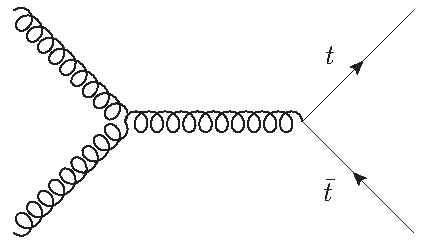
\includegraphics[width=0.32\textwidth]{figs/Gluon_fusion_top_pair.jpg}
    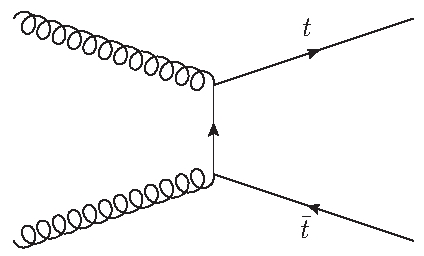
\includegraphics[width=0.32\textwidth]{figs/Gluon_tchannel_top_pair.jpg}
    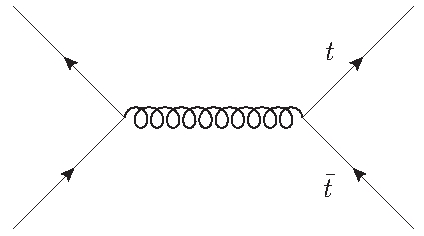
\includegraphics[width=0.32\textwidth]{figs/Quarks_schannel_top_pair.jpg}
    \caption{Top pair production processes Feynman diagrams for proton-proton collisions, via gluon fusion and quark-antiquark annihilation}
    \label{fig:PairProduction}
  \end{center}
\end{figure}

\begin{figure}[!Hhtbp]
  \begin{center}
    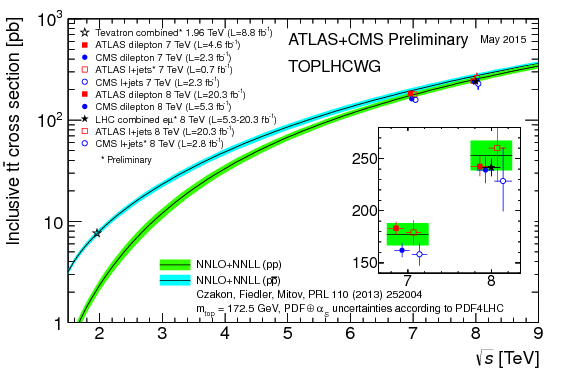
\includegraphics[width=0.9\textwidth]{figs/toplhcwg_ttxsec_sqrts_may2015.png}
    \caption{$t\bar{t}$ production cross section as function of the center of mass energy in $p\bar{p}$ and $pp$ collisions compared to theoretical predictions.}
    \label{fig:PairProduction}
  \end{center}
\end{figure}

%\begin{TOINCLUDE}Plots of cross section of ttbar production as function of center of mass energy; Feynman diagrams for pair production\end{TOINCLUDE}

\subsection{Single $t$ production}
\label{subsec:topsing}

Description of single production and the relative importance of each channel.

\begin{figure}[!Hhtbp]
  \begin{center}
    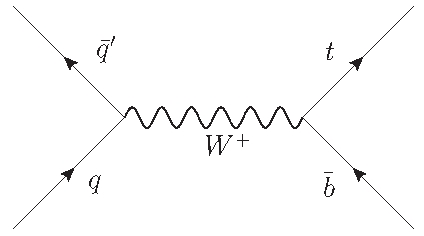
\includegraphics[width=0.32\textwidth]{figs/Schannel_top_single.jpg}
    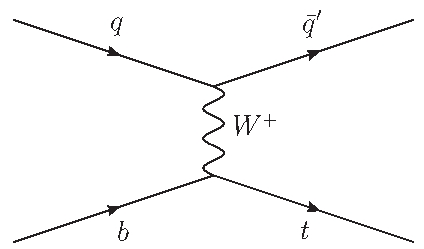
\includegraphics[width=0.32\textwidth]{figs/Tchannel_top_single.jpg}
    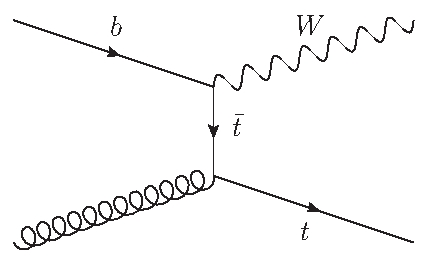
\includegraphics[width=0.32\textwidth]{figs/TWchannel_top_single.jpg}
    \caption{Single top production processes Feynman diagrams for proton-proton collisions, from left to right s-channel, t-channel and associated $W$ production.}
    \label{fig:PairProduction}
  \end{center}
\end{figure}

\begin{figure}[!Hhtbp]
  \begin{center}
    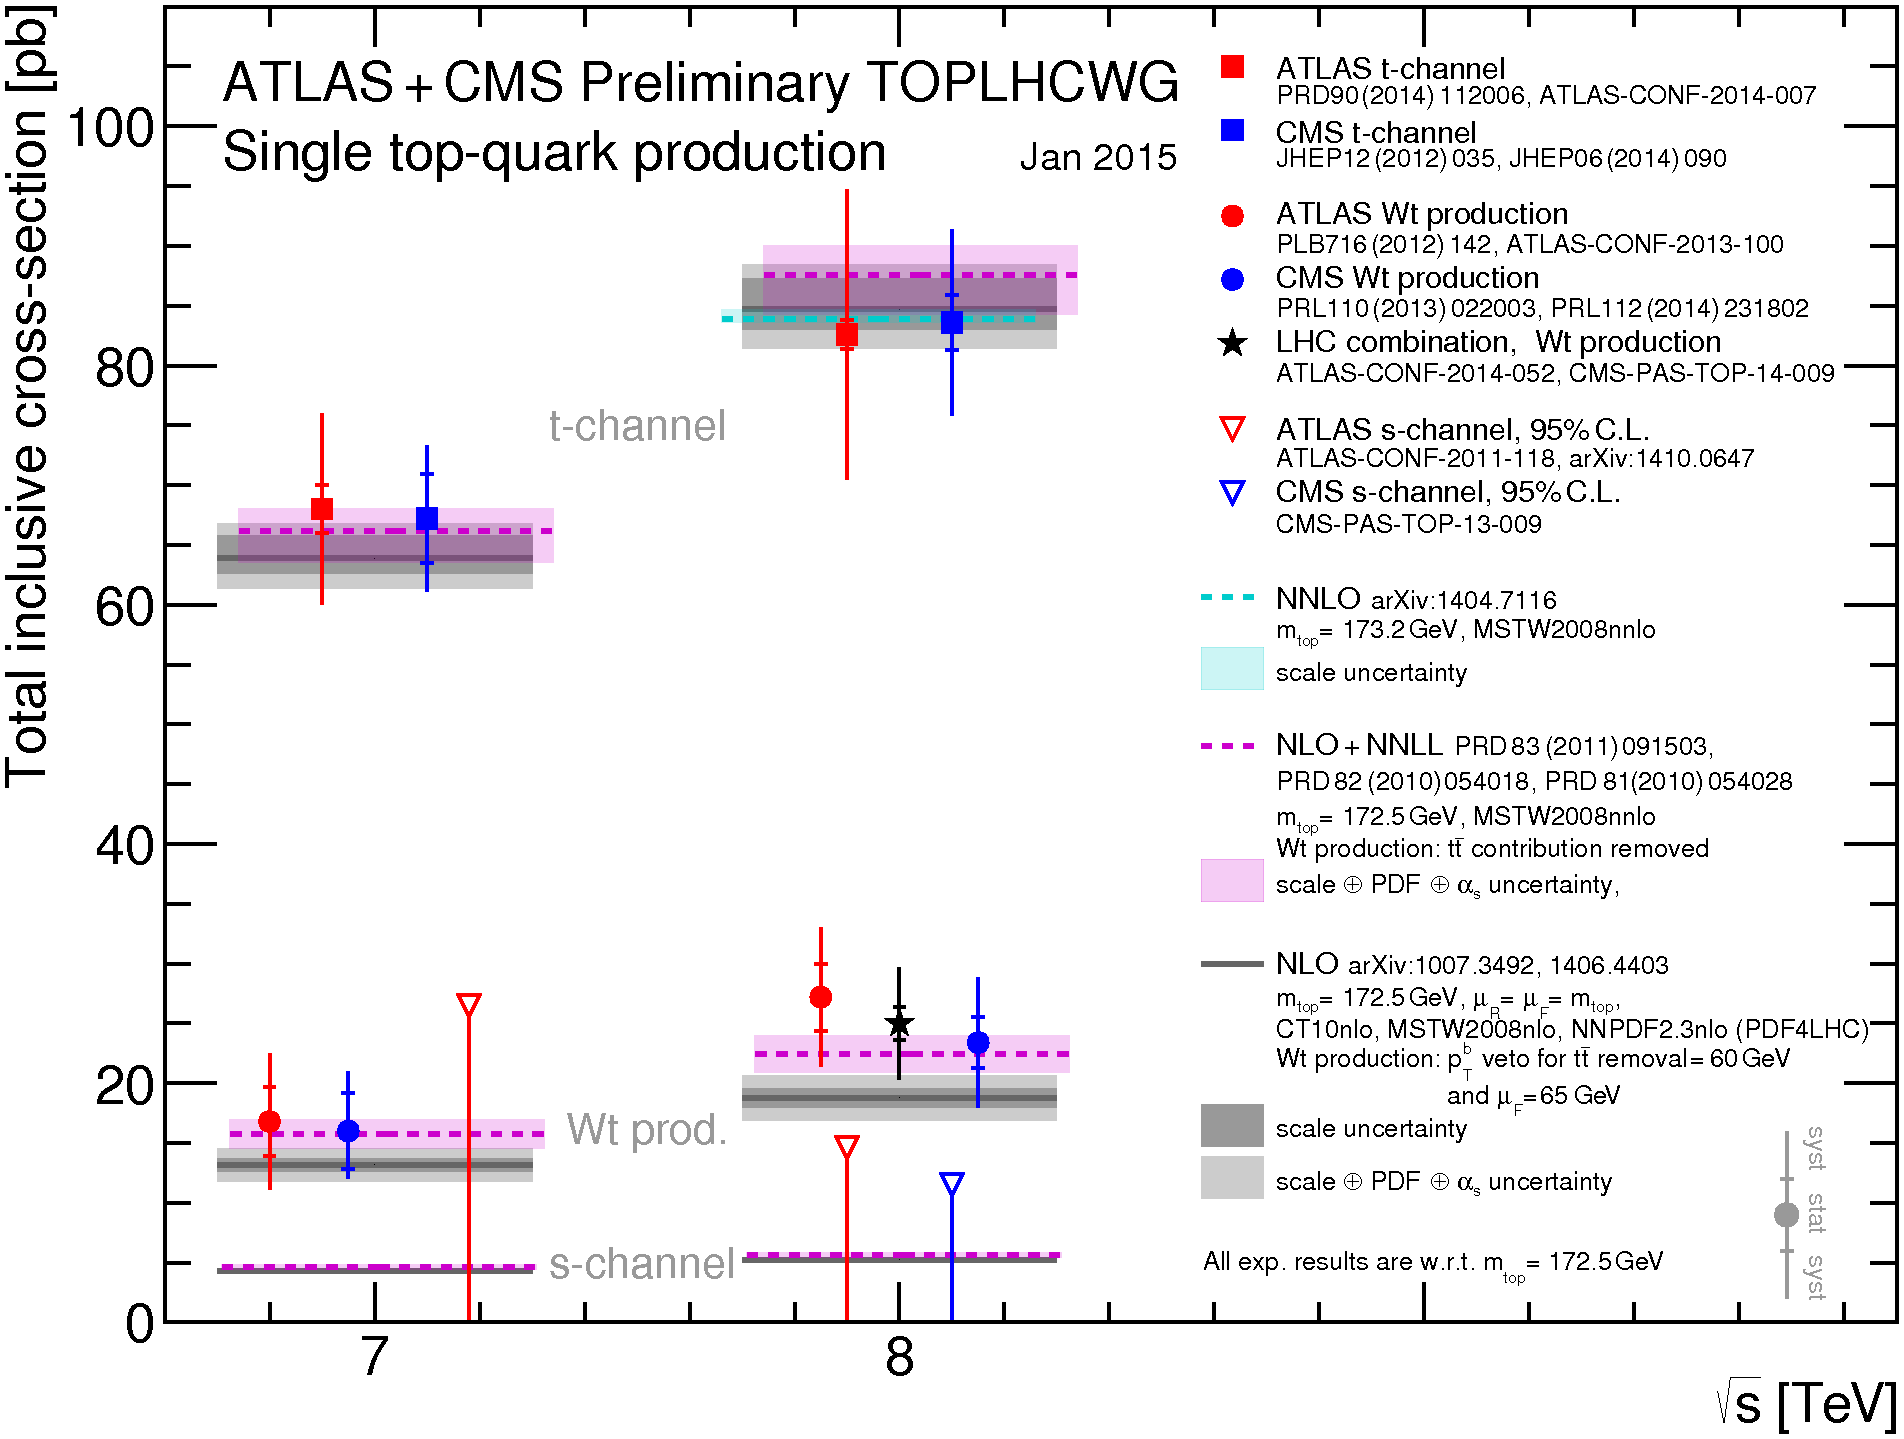
\includegraphics[width=0.9\textwidth]{figs/singletop_allchanvsroots.png}
    \caption{Single top production cross section as function of the center of mass energy in $pp$ collisions compared to theoretical predictions for each production channel by ATLAS and CMS collaborations.}
    \label{fig:PairProduction}
  \end{center}
\end{figure}

%\begin{TOINCLUDE}Plots of cross section of single-top production as function of center of mass energy; Feynman diagrams for single production\end{TOINCLUDE}

\subsection{Decay channels}

Description of possible decays of top-quark to show different channels of searches.

\begin{figure}[!Hhtbp]
  \begin{center}
    
\includegraphics[width=0.3\textwidth]{figs/CMSlogo.png}
    \caption{Feynman diagrams for top decay channels with respective branching ratios.}
    \label{fig:BRratiosandDecayChannels}
  \end{center}
\end{figure}

%\begin{TOINCLUDE}Plot on possible decay channels and branching ratios to each channel; Feynman diagram for each decay channel\end{TOINCLUDE}

\subsection{Top properties}

Description of top properties and the measurement of them.

\subsubsection{Electric charge}

Top charge related to its decay.

\subsubsection{Lifetime}

Discussion on the importance of measurements of top as only quark decaying before hadronization time.

\subsubsection{Mass and width}

Measurements of top mass and width.

\begin{figure}[!Hhtbp]
  \begin{center}
    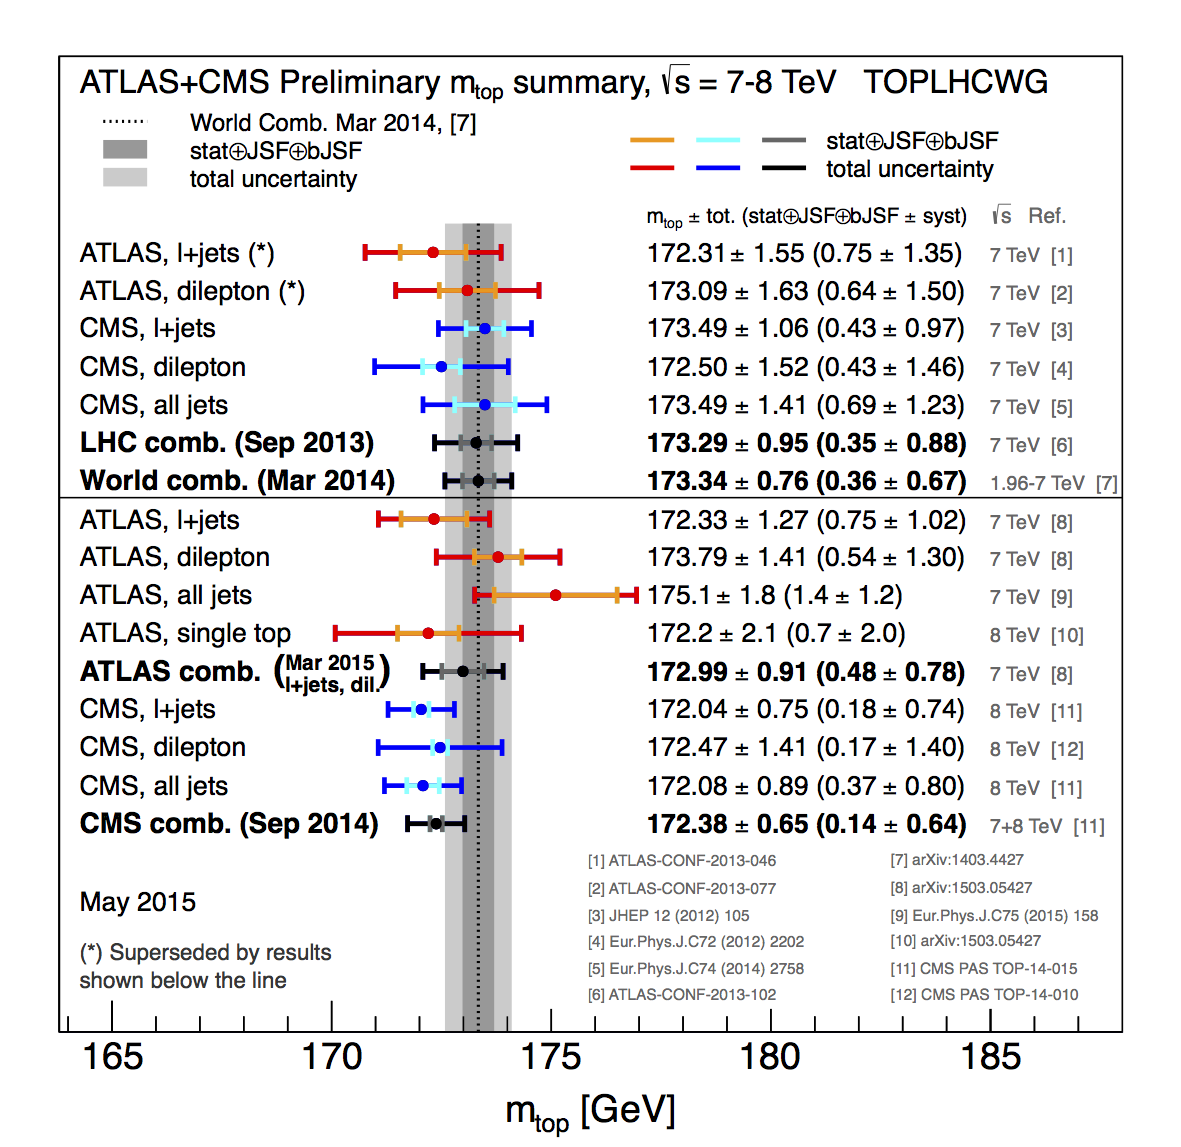
\includegraphics[width=0.9\textwidth]{figs/LHC_topmass_May2015.png}
    \caption{Top mass measurements from ATLAS and CMS collaborations and world combination including Tevatron results.}
    \label{fig:TopMass}
  \end{center}
\end{figure}

%\begin{TOINCLUDE}Plot of top mass measurement from Tevatron+LHC combination\end{TOINCLUDE}

\subsubsection{Spin correlation}

Discussion on how ttbar system have spin correlation that will be important for precision measurements.

\section{Higgs production at LHC}

Discussion of Higgs production channels and relative importance.

\begin{figure}[!Hhtbp]
  \begin{center}
    
\includegraphics[width=0.3\textwidth]{figs/CMSlogo.png}
    \caption{Higgs production Feynman diagrams for proton-proton collisions.}
    \label{fig:HiggsProd}
  \end{center}
\end{figure}

\begin{figure}[!Hhtbp]
  \begin{center}
    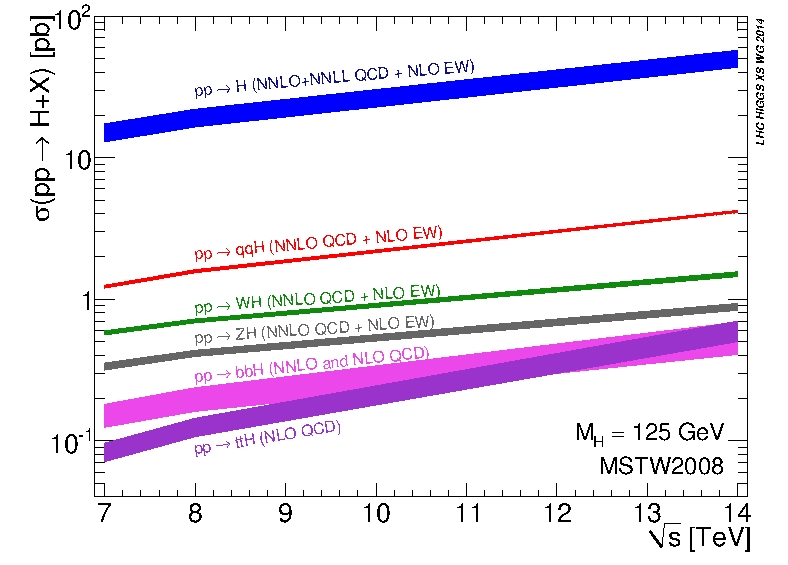
\includegraphics[width=0.8\textwidth]{figs/7-14_Higgs_xsec.jpg}
    \caption{Higgs production cross section theoretical predictions as function of center of mass energy.}
    \label{fig:HiggsProdXS}
  \end{center}
\end{figure}

%\begin{figure}[!Hhtbp]
%  \begin{center}
%    
\includegraphics[width=0.3\textwidth]{figs/CMSlogo.png}
%    \caption{}
%    \label{fig:}
%  \end{center}
%\end{figure}

%\begin{TOINCLUDE}Plots of cross section of Higgs production as function of center of mass energy; Feynman diagrams for Higgs production\end{TOINCLUDE}

\subsection{Decay channels}

Discussion of Higgs decays and relative importance also related to the resolution of channels.

\begin{figure}[!Hhtbp]
  \begin{center}
    
\includegraphics[width=0.3\textwidth]{figs/CMSlogo.png}
    \caption{Feynman diagrams of Higgs decay: $b\bar{b}$ [left], diphoton [center] and golden channels [right]}
    \label{fig:HiggsDecays}
  \end{center}
\end{figure}

\begin{figure}[!Hhtbp]
  \begin{center}
    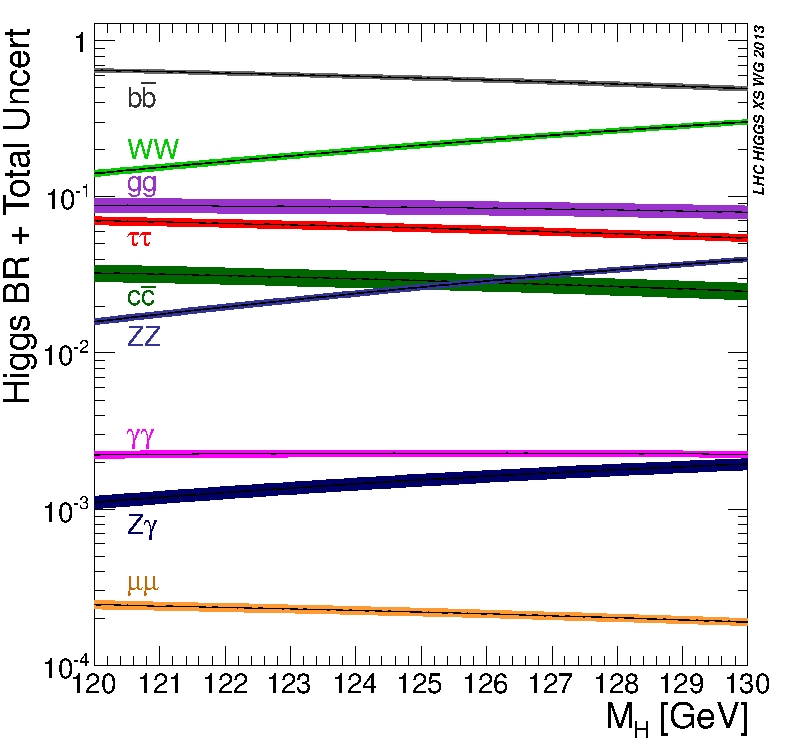
\includegraphics[width=0.8\textwidth]{figs/Higgs_BR_120-130.jpg}
    \caption{Higgs decay branching ratios.}
    \label{fig:HiggsBrs}
  \end{center}
\end{figure}
%\begin{TOINCLUDE}Plot on possible decay channels and branching ratios to each channel; Feynman diagram for each golden bb and diphoton channels\end{TOINCLUDE}

\subsection{Higgs properties}

\subsubsection{Electric charge}

Higgs neutrality description.

\subsubsection{Spin}

Importance of spin parity determination to know if it's the SM one. 

\begin{figure}[!Hhtbp]
  \begin{center}
    
\includegraphics[width=0.3\textwidth]{figs/CMSlogo.png}
    \caption{Higgs spin parity measurement}
    \label{fig:HiggsSpinParity}
  \end{center}
\end{figure}
%\begin{TOINCLUDE}Plot on spin-parity measurement of Higgs boson\end{TOINCLUDE}

\subsubsection{Mass and width}

Mass and width measurements.

\begin{figure}[!Hhtbp]
  \begin{center}
    
\includegraphics[width=0.3\textwidth]{figs/CMSlogo.png}
    \caption{ATLAS and CMS combination of Higgs mass measurement [left] and signal strength for searches performed by CMS in different Higgs channels [right]}
    \label{fig:HiggsMass}
  \end{center}
\end{figure}

\begin{figure}[!Hhtbp]
  \begin{center}
    
\includegraphics[width=0.3\textwidth]{figs/CMSlogo.png}
    \caption{Higgs mass observation by CMS collaboration in the diphoton [left] and golden channels [right].}
    \label{fig:MassDiphotonMassGolden}
  \end{center}
\end{figure}

%\begin{figure}[!Hhtbp]
%  \begin{center}
%    
\includegraphics[width=0.3\textwidth]{figs/CMSlogo.png}
%    \caption{}
%    \label{fig:}
%  \end{center}
%\end{figure}
%\begin{TOINCLUDE}Plot on ATLAS+CMS combination of the Higgs mass; Plot on signal strength for each decay channel; Individual plots on diphoton channel and golden channel\end{TOINCLUDE}

\section{Hierarchy problem and other limitations}
\label{sec:hier}

The SM has been one of the most successful theories on the history of physics. With only 19 free parameters, is able to make thousands of predictions that have been measured and tested over the last seventy to eighty years. However some aspects in the model are not completely understood. The most important one is the so-called hierarchy mass problem. At tree level, the Englert-Brout-Higgs boson has a mass $m_{H}^{2}=-2\mu^{2}$, but the physical mass also contain the one-loop contributions from fermions that interact with it, as the top quark. The Feynman diagram for such contribution can be seen in figure~\ref{fig:oneloophiggs}.

\begin{figure}[!Hhtbp]
  \begin{center}
    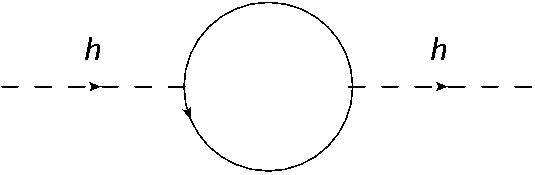
\includegraphics[width=0.6\textwidth]{figs/HierarchyLoop.png}
    \caption{One loop diagram for contributions to the mass of the Englert-Brout-Higgs boson from interactions with fermions}
    \label{fig:oneloophiggs}
  \end{center}
\end{figure}

Such contributions add up giving a mass greater than simple tree level mass. Each fermion contributes proportionally to its mass, what means that the top quark contributes the most. Moreover, if there are in nature heavier fermions that also interact with the Englert-Brout-Higgs boson they will also contribute to its mass. With such considerations one can expect the Englert-Brout-Higgs boson to be much greater than 125 GeV, and in principle not even of the order of 100 GeV but greater than 1 TeV. However the real relevance or significance of this problem at theoretical level has been discussed extensively, for example at~\cite{Jegerlehner:2013nna}, the majority of the community agrees there is something to be understood on the subject. 

The most famous proposed solution to this problem is supersymmetry (SUSY)~\cite{Martin:1997ns}. It proposes the existence of an additional symmetry between fermions and bosons, at a given point of the history of universe nature didn't distinguish between fermions and bosons. However, we know this does not happen at the present, and then this symmetry should be broken. Such symmetry implies the existence of a super-symmetric partner for each particle, a super-partner. A fermion for each boson and vice versa. This SUSY procedure doubles the particle content of the model where it's applied. Before breaking SUSY, a particle and it's partner have the same mass. In this feature is where the hierarchy problem is solved. On figure~\ref{fig:susy} one can see the one loop diagrams for the mass of the Englert-Brout-Higgs boson from the top and its super-partner the stop. Whereas, the top contribution is positive, the stop contribution is negative but equal in value, then cancelling between them.

\begin{figure}[!Hhtbp]
  \begin{center}
    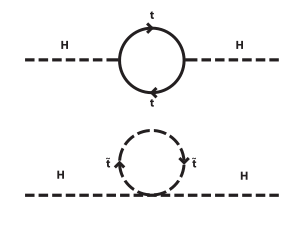
\includegraphics[width=0.6\textwidth]{figs/SUSY.png}
    \caption{One loop diagrams for contributions to the mass of the Englert-Brout-Higgs boson from the top and the stop}
    \label{fig:susy}
  \end{center}
\end{figure}

But this solution works exactly only if SUSY is not broken. As we know SUSY has to be broken, there has been developed in the literature different ways to brake SUSY and still offer a solution to the hierarchy problem, leading normally to solutions that need a fine adjustment of the parameters of the theory. This represents for some theoreticians a problem itself: Fine-tuning or Naturalness. Extensive searches for SUSY particles have been performed, accordingly to different model realizations MSSM~\cite{Khachatryan:2014wca,Aad:2014vgg}, CMSSM, etc.

While hierarchy problem is an internal problem of the SM, there are several questions that have not been solved. For example, how gravity is understood in the frame of QFT's, why there is only 3 generations of leptons and quarks, why there is only 4 fundamental forces among others. In addition, there have been experimental questionings to the SM. The mos important one is the masses of neutrinos. In the SM neutrinos are massless, careful measurements,~\cite{Ashie:2004mr, Weinheimer:2013hya}, have shown that neutrinos can oscillate between different flavors, phenomenon only possible if neutrinos have a mass. Measurements of solar and atmospheric neutrino oscillations have been the most important proof of physics beyond the SM. 

From cosmological measurements, the Wilkinson Microwave Anisotropy Probe have shown that the universe is not only made by visible matter, but suggests that around 24\% its made of dark matter. A type of matter not visible by means of light. It has also shown that 71\% of the universe is composed of dark energy, what makes the universe to be in an accelerated state of expansion. These results can be seen in~\cite{2013ApJS..208...20B, 2013ApJS..208...19H}. Also the Planck probe has shown similar results, for example in~\cite{Planck:2015xua}. The SM does not have any answer to this open problems so far. 

Finally, there is known that the universe presents an asymmetry between matter and antimatter, being the first much more abundant than the second. Such asymmetry can be obtained by CP-violating processes (C for charge and P for parity). However the amount of CP violation present in the SM is not compatible with the huge matter-antimatter asymmetry in nature. This problem, known as baryon asymmetry, represent an additional huge challenge for particle physics. 

In conclusion, the SM has been a formidable model that has helped us to understand a huge amount of physics. It has done thousands of predictions that have been measured and corroborated one by one in the last half-century. However, this is not the end of the story, perhaps only the beginning. There are theoretical and experimental motivations that lead us think that the SM is not the ``final'' theory that could explain all subatomic phenomena in nature. Currently, there is a mayor effort, both theoretical and experimentally, to understand and explain all the remaining pieces. The present work is one of them.

In the next chapter, we present an extension of the SM that looks for a solution to the discussed hierarchy problem.